\section{Introduction}
\label{sec:intro}

\begin{figure}[t]
  \centering
  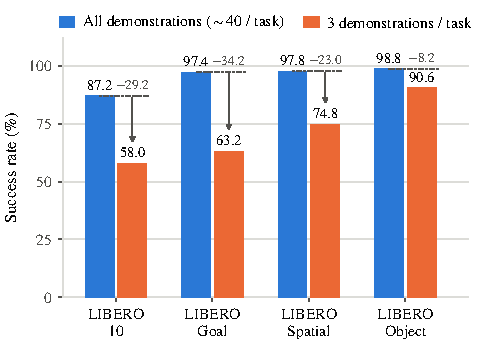
\includegraphics[width=\linewidth]{fig/fig1_data_scarcity.pdf}
  \caption{\textbf{Few-shot post-training collapses.}
  Closed-loop success rate of the pre-trained \base model after post-training on all demonstrations of each LIBERO suite (blue; 379--454 demonstrations, about 40 per task) and on three demonstrations per task (orange; 30 per suite), with the post-training recipe otherwise identical.
  The same recipe loses 8 to 34 points when demonstrations are scarce.
  Every bar is 50 trials on each of the 10 tasks of a suite.}
  \label{fig:teaser}
\end{figure}

Progress in artificial intelligence over the past decade has followed a simple pattern: large models are pre-trained on broad data and then adapted to a target task from comparatively little data.
Robot learning has adopted the same pattern.
Vision-language-action models (VLAs)~\cite{zitkovich2023rt2,kim2024openvla,black2024pi0,nvidia2025groot} and, more recently, world action models (WAMs) that generate future video and robot actions jointly~\cite{du2023unipi,wu2024gr1,zhu2025uwm,cen2025worldvla,cosmos3} are pre-trained on web-scale video and cross-embodiment robot data~\cite{oneill2024oxe,khazatsky2024droid}, and are then \emph{post-trained} on demonstrations collected with the target robot in the target environment, where an action objective turns the pre-trained network into a policy.
When the post-training set is large, the recipe is remarkably effective.
On the four LIBERO suites~\cite{liu2023libero}, post-training the pre-trained \base model~\cite{cosmos3} on all available demonstrations reaches 87--99\% success (\cref{fig:teaser}, blue).

Demonstrations, however, are the most expensive ingredient of this pipeline.
Every new robot, workcell, or task requires a person to teleoperate it, and in many deployments only a handful of demonstrations per task is affordable.
In this regime the standard recipe breaks down.
With very few demonstrations per task, the same post-training recipe loses between 8 and 34 points on the four LIBERO suites (\cref{fig:teaser}, orange), and the loss is largest on the long-horizon and the goal-conditioned suites.
A model that has been pre-trained on millions of robot and human videos does not turn a few demonstrations into a reliable policy.

We attribute this gap to a mismatch between what pre-training optimizes and what few-shot post-training needs.
Pre-training optimizes the weights for the \emph{joint} objective over a mixture of embodiments and tasks, and nothing in that objective asks the weights to be a good \emph{starting point} for a short fine-tune on an embodiment outside the mixture.
Being good at many embodiments and adapting effectively to a new one from few demonstrations are different properties, and a pre-trained model that has the first does not automatically have the second.
A second, complementary effect appears during post-training itself.
With only a few demonstrations, the policy latches onto the visual context of each demonstration, which already identifies the task in most benchmarks, and largely ignores the language instruction; in scenes that are shared by several tasks it then executes the wrong task.

We address the first problem with \Method, a stage inserted between the existing pre-training and post-training (\cref{fig:method}).
The stage builds episodes from five robot datasets of different embodiments, each episode simulating the downstream problem: a few demonstrations of one source embodiment and a short fine-tuning on them.
After each episode, the weights are moved a fraction of the way toward the adapted solution, following first-order meta-learning~\cite{nichol2018reptile}.
Because this update is a plain interpolation in weight space, the entire trainable set of the post-training recipe can be meta-trained with the standard training stack, and the resulting checkpoint is a drop-in replacement for the pre-trained weights: post-training proceeds exactly as before, only from a better starting point.
We address the second problem with \Rpl (\RPL), a post-training objective that samples negative instructions and requires the action prediction under a wrong instruction to be worse than under the correct one, which forces the policy to commit to the instructed behavior rather than to the behavior suggested by the scene.

On the four LIBERO suites with three demonstrations per task, our approach raises the average success rate from 71.7\% to 78.7\%, with gains of 11.4 points on LIBERO-10 and 13.0 points on LIBERO-Goal, and improves every one of the ten LIBERO-10 tasks.
Ordinary training on the same source datasets yields no gain (58.0\% to 58.2\% on LIBERO-10), so the improvement comes from meta-learning rather than from additional data.
The meta pre-trained initialization also helps when data is plentiful: with all LIBERO-10 demonstrations the success rate rises from 87.2\% to 94.6\%.
In summary, our contributions are:
\begin{itemize}
  \item We identify and quantify the few-shot post-training problem of pre-trained robot policies on the four LIBERO suites, where the standard recipe loses 8--34 points when only a few demonstrations per task are available.
  \item We propose \Method, a stage between pre-training and post-training that optimizes the entire trainable set of the post-training recipe for few-shot adaptation while leaving the architecture and the post-training recipe unchanged, and \Rpl, a post-training objective that counteracts the visual bias of few-shot policies.
  \item We show consistent gains in the few-shot regime, a control experiment in which ordinary training on the same source data gives none, and a gain in the full-data regime.
\end{itemize}
